\documentclass[12pt]{article}
\usepackage[a4paper]{geometry}
\usepackage[utf8]{inputenc}
\usepackage{fancyhdr}
\usepackage{lastpage}
\usepackage{graphicx, wrapfig, subcaption, setspace, booktabs}
\usepackage{graphicx}
\usepackage[T1]{fontenc}
\usepackage[font=small, labelfont=bf]{caption}
\usepackage[protrusion=true, expansion=true]{microtype}
\usepackage[english]{babel}
\usepackage{sectsty}
\usepackage{url, lipsum}
\usepackage[T1]{fontenc}
\usepackage{icomma}
\usepackage{siunitx}
\usepackage{ragged2e}
\usepackage{amsmath}
\usepackage{comment}
\usepackage{enumerate}
\usepackage{anysize}

\newcommand{\HRule}[1]{\rule{\linewidth}{#1}}
\onehalfspacing
\setcounter{tocdepth}{5}
\setcounter{secnumdepth}{5}

%-------------------------------------------------------------------------------
% HEADER & FOOTER
%-------------------------------------------------------------------------------


\begin{comment}
-Udledninger
$$
\begin{aligned}
\end{aligned}
$$

-Opgavetekst
\begin{figure}[H]
\includegraphics[width=0.5\textwidth]{"path"}
\end{figure} 


-Opgave billede med tekst
\begin{figure}[H]
\caption{"Billedtekst"}
\includegraphics[width=0.5\textwidth]{"path"}
\end{figure} 

-Værdier
$\\
$


\end{comment}
\begin{document}

\begin{titlepage}

\title{ \normalsize 
		%\begin{figure}
        \begin{center}
        
\includegraphics[height=6cm]{Logo.jpg}
        \end{center}
       % \end{figure}
        \LARGE \textsc{\textbf{Universidad De Sonora}} \\ \bigskip
		\Large División de Ciencias Exactas y Naturales \\
        Licenciatura en Física \\ \bigskip
        \bigskip
        Física Computacional I
		\\ [0.1cm]  
		\HRule{2pt} \\
		\Large \textbf{{Actividad 9}} \\
        \textit{\textbf{"Teoría de Estabilidad de las Soluciones de las Ecuaciones Diferenciales Ordinarias"}}
		\HRule{2pt} \\
		\normalsize \vspace*{0.001\baselineskip}}
        
\date{\bigskip \Large  \hspace*{\fill} Hermosillo, Sonora a abril 06 de 2021}

        
\author{
		\Large\textbf{Ismael Espinoza Arias} \\ \bigskip
        \\ \bigskip
       \Large Profesor Carlos Lizárraga Celaya}
       \end{titlepage}
       \maketitle
       
       
%-----------------------------------------------------------


\section*{Introducción y Antecedentes}
En matemáticas, la teoría de estabilidad estudia la estabilidad de las soluciones de ecuaciones diferenciales y sistemas dinámicos, es decir, examina cómo difieren las soluciones bajo pequeñas modificaciones de las condiciones iniciales.\\

La estabilidad es muy importante en física y ciencias aplicadas, ya que en general en los problemas prácticos las condiciones iniciales nunca se conocen con toda precisión, y la predictibilidad requiere que pequeñas desviaciones iniciales, no generen comportamientos cualitativamente muy diferentes a corto plazo. Cuando la diferencia entre dos soluciones con valores iniciales cercanos puede acotarse mediante la diferencia de valores iniciales, se dice que la evolución temporal del sistema presenta estabilidad.\\




%-----------------------------------------------------------


\section*{Estabilidad de ecuaciones diferenciales}

Debido a que toda ecuación diferencial puede reducirse a un sistema de ecuaciones diferenciales de primer orden equivalente, el estudio de la estabilidad de las soluciones de ecuaciones diferenciales puede reducirse al estudio de la estabilidad de los sistemas de ecuaciones diferenciales. Consideremos por ejemplo un sistema de ecuaciones autónomo no lineal dado por:

\begin{center}
    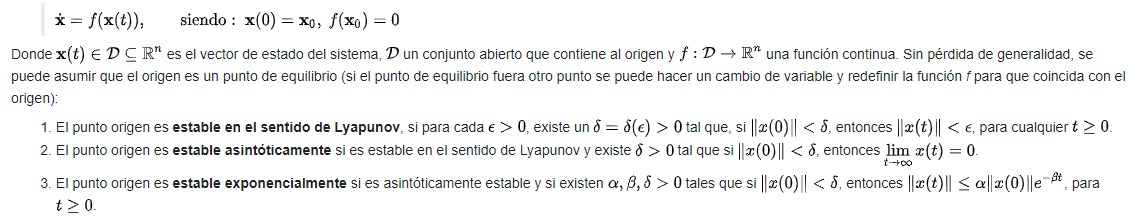
\includegraphics[height=3.2cm]{I1.jpeg}
\end{center}


%-----------------------------------------------------------


\subsection*{Importación de bibliotecas}
Empezamos importando nuestras bibliotecas, el primer paso para empezar con cualqueir actividad.

\begin{center}
    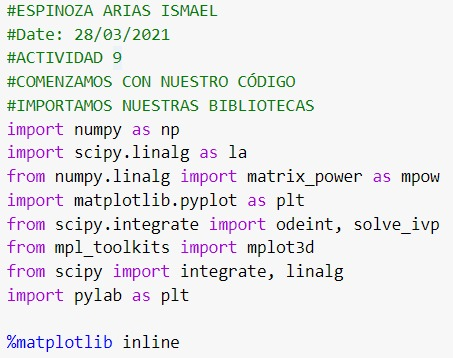
\includegraphics[height=13cm]{I2.jpeg}
\end{center}
 
 Donde podemos ver que las bibliotecas utilizadas, son numpy, scipy, matplotlib, pylab, ect.


%-----------------------------------------------------------


\subsection*{Realización de la actividad}
Ahora para la actividad, vamos a definir nuestros valores, asi como los vectores, matrices, eigenvectores, entre otrás cosas más.

\begin{center}
    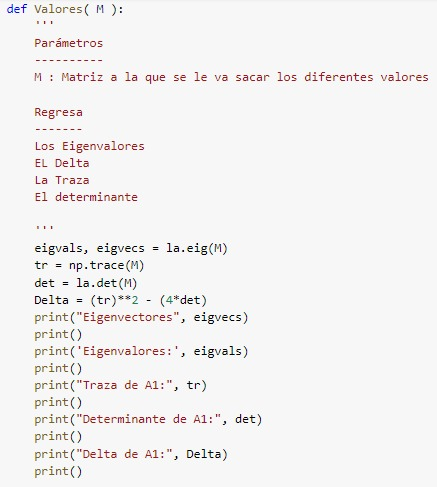
\includegraphics[height=18cm]{I3.jpeg}
\end{center}
 

%-----------------------------------------------------------


\subsection*{Ejercicio 1}
llegamos al siguiente ejercicio.

\begin{center}
    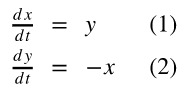
\includegraphics[height=5cm]{E1.jpeg}
\end{center}

Tenemos que la soluciones són:

\begin{center}
    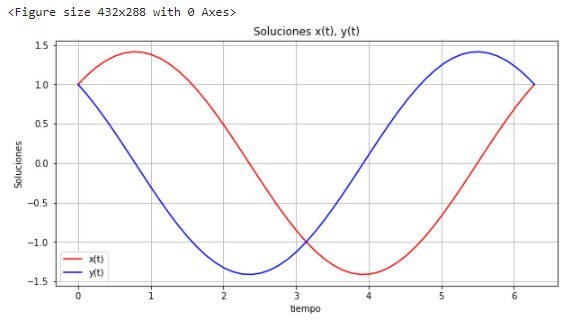
\includegraphics[height=9cm]{S1.jpeg}
\end{center}

Solución en el estado fase:

\begin{center}
    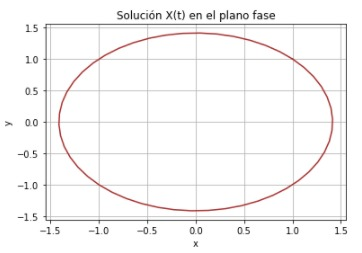
\includegraphics[height=9cm]{S12.jpeg}
\end{center}


%-----------------------------------------------------------


\subsection*{Ejercicio 2}
llegamos al siguiente ejercicio.

\begin{center}
    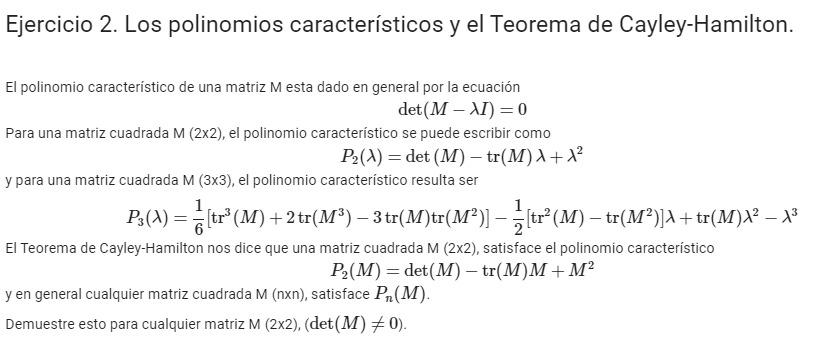
\includegraphics[height=5cm]{E2.jpeg}
\end{center}

Tenemos que la soluciones són:

\begin{center}
    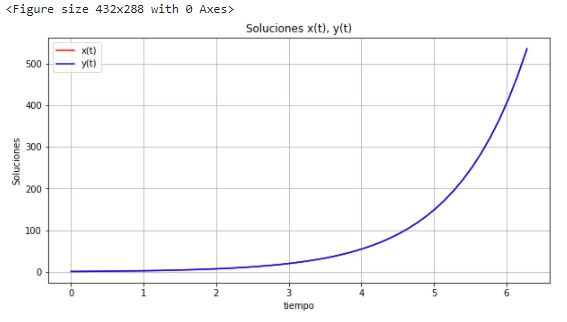
\includegraphics[height=9cm]{S2.jpeg}
\end{center}

Solución en el estado fase:

\begin{center}
    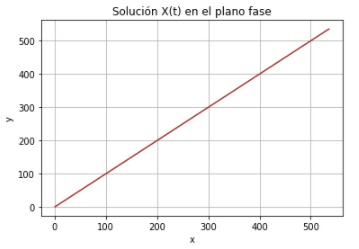
\includegraphics[height=9cm]{S22.jpeg}
\end{center}


%-----------------------------------------------------------


\subsection*{Ejercicio 3}
llegamos al siguiente ejercicio.

\begin{center}
    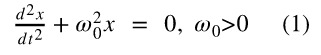
\includegraphics[height=3cm]{E3.jpeg}
\end{center}

Tenemos que la soluciones són:

\begin{center}
    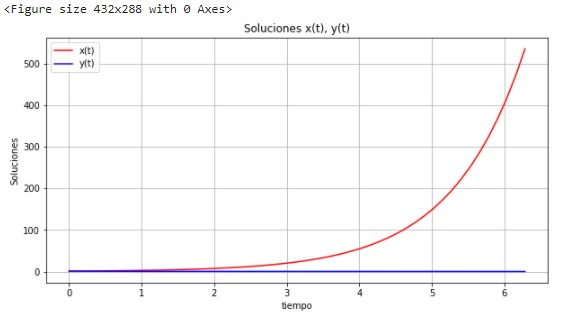
\includegraphics[height=9cm]{S3.jpeg}
\end{center}

Solución en el estado fase:

\begin{center}
    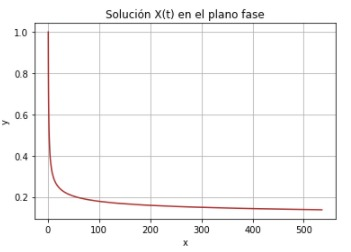
\includegraphics[height=9cm]{S33.jpeg}
\end{center}


%-----------------------------------------------------------


\subsection*{Ejercicio 4}
llegamos al siguiente ejercicio.

\begin{center}
    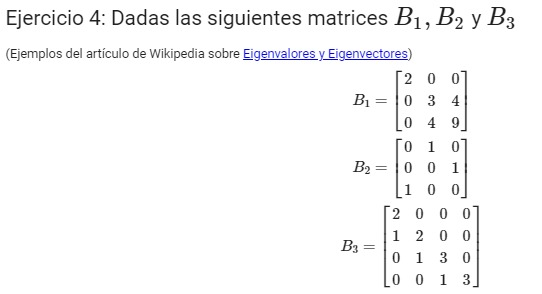
\includegraphics[height=6cm]{E4.jpeg}
\end{center}

Tenemos que la soluciones són:

\begin{center}
    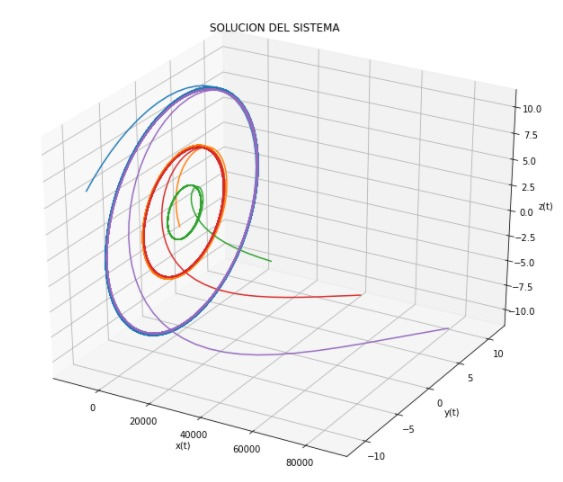
\includegraphics[height=12cm]{S4.jpeg}
\end{center}


%-----------------------------------------------------------


\subsection*{Ejercicio 5}
llegamos al siguiente ejercicio.

\begin{center}
    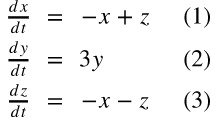
\includegraphics[height=5cm]{E5.jpeg}
\end{center}

Tenemos que la soluciones són:

\begin{center}
    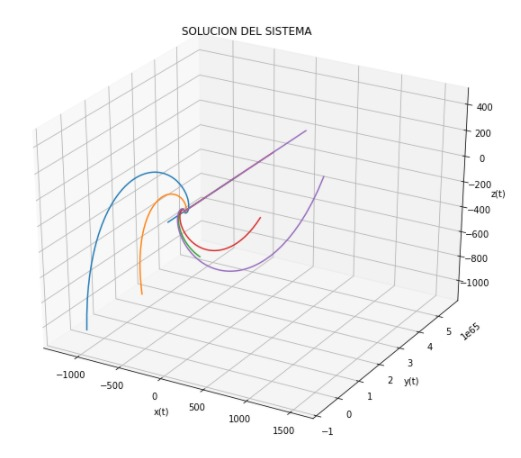
\includegraphics[height=12cm]{S5.jpeg}
\end{center}


%-----------------------------------------------------------


\subsection*{Ejercicio 6}
llegamos al siguiente ejercicio.

\begin{center}
    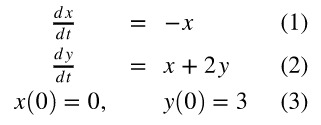
\includegraphics[height=5cm]{E6.jpeg}
\end{center}

Tenemos que la soluciones són:

\begin{center}
    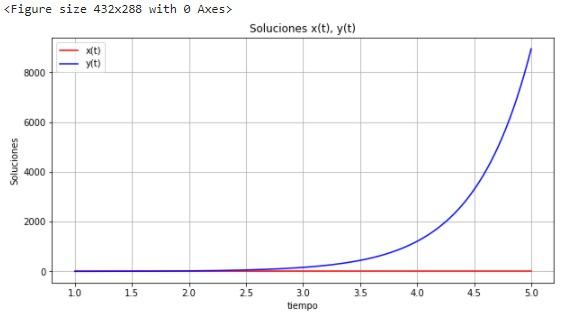
\includegraphics[height=9cm]{S6.jpeg}
\end{center}

Solución en el estado fase:

\begin{center}
    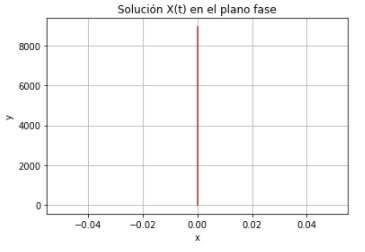
\includegraphics[height=9cm]{S66.jpeg}
\end{center}


%-----------------------------------------------------------


\subsection*{Ejercicio 7}
llegamos al siguiente ejercicio.

\begin{center}
    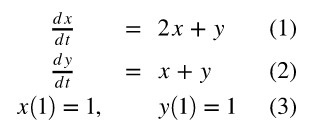
\includegraphics[height=5cm]{E7.jpeg}
\end{center}

Tenemos que la soluciones són:

\begin{center}
    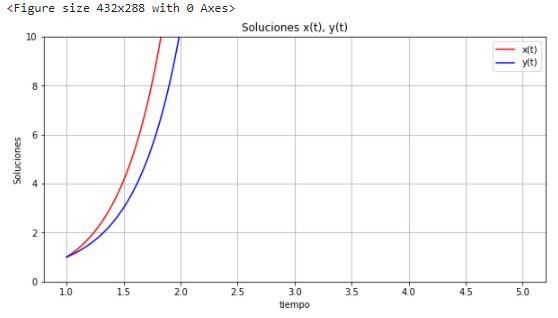
\includegraphics[height=9cm]{S7.jpeg}
\end{center}

Solución en el estado fase:

\begin{center}
    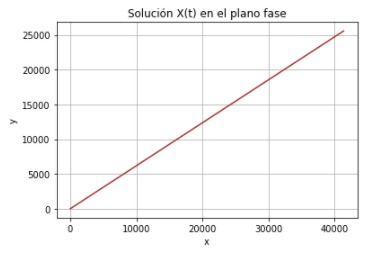
\includegraphics[height=9cm]{S77.jpeg}
\end{center}


%-----------------------------------------------------------


\subsection*{Ejercicio 8}
llegamos al siguiente ejercicio.

\begin{center}
    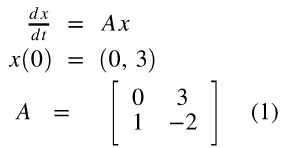
\includegraphics[height=5cm]{E8.jpeg}
\end{center}

Tenemos que la soluciones són:

\begin{center}
    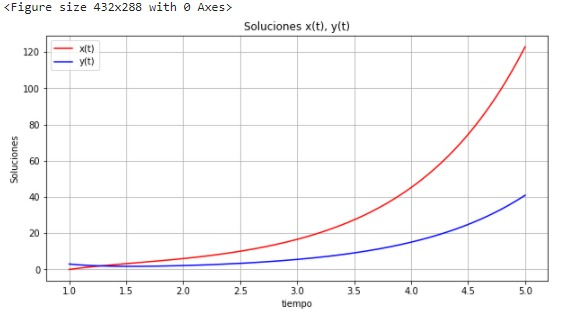
\includegraphics[height=9cm]{S8.jpeg}
\end{center}

Solución en el estado fase:

\begin{center}
    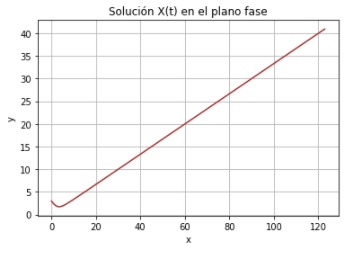
\includegraphics[height=9cm]{S88.jpeg}
\end{center}


%-----------------------------------------------------------


\subsection*{Ejercicio 9}
llegamos al siguiente ejercicio.

\begin{center}
    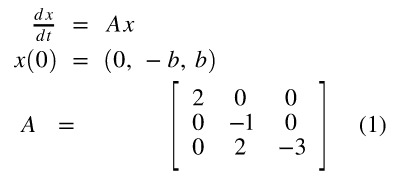
\includegraphics[height=5cm]{E9.jpeg}
\end{center}

Tenemos que la soluciones són:

\begin{center}
    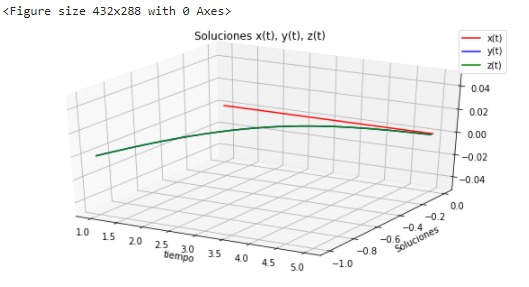
\includegraphics[height=9cm]{S9.jpeg}
\end{center}

Solución en el estado fase:

\begin{center}
    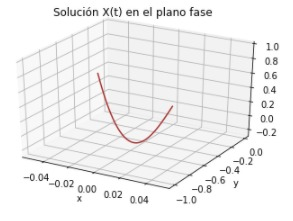
\includegraphics[height=9cm]{S99.jpeg}
\end{center}


%-----------------------------------------------------------

\subsection*{Ejercicio 10}
llegamos al siguiente ejercicio.

\begin{center}
    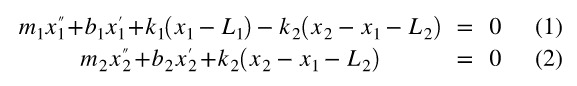
\includegraphics[height=2cm]{E10.jpeg}
\end{center}

Solución en el estado fase:

\begin{center}
    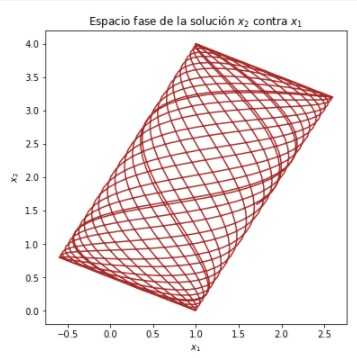
\includegraphics[height=10cm]{S10.jpeg}
\end{center}

Gráfico:

\begin{center}
    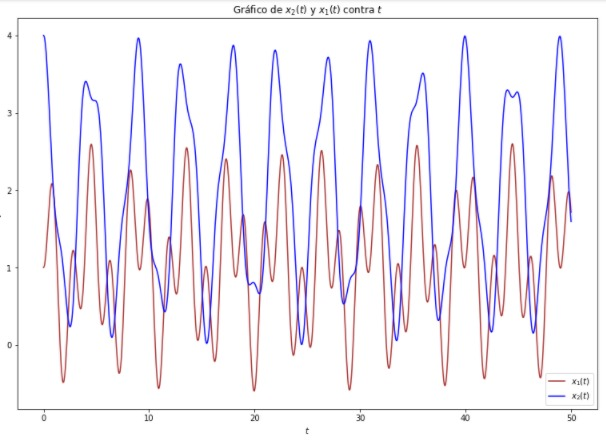
\includegraphics[height=10cm]{S1010.jpeg}
\end{center}

Solución en el estado fase:

\begin{center}
    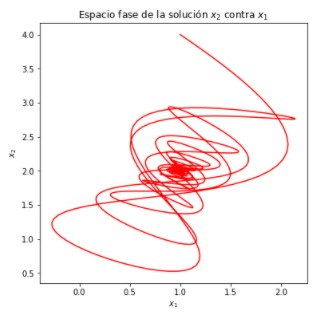
\includegraphics[height=10cm]{S11.jpeg}
\end{center}

Gráfico:

\begin{center}
    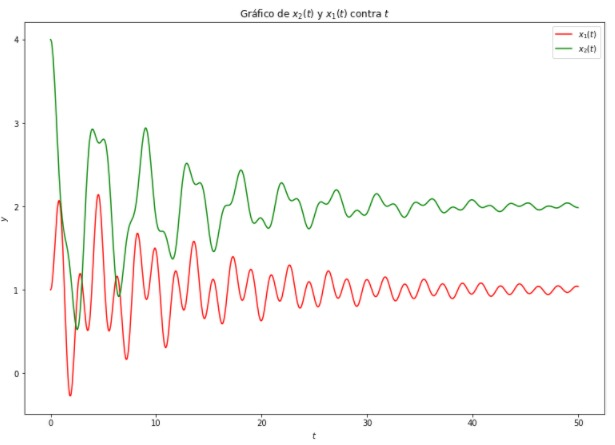
\includegraphics[height=10cm]{S1111.jpeg}
\end{center}




%-----------------------------------------------------------


\section*{Resultados y Discusión}
Como nos pudimos dar cuenta las gráficas se hacen de una distinta, es decir, dependen de ciertas cosas para realizarlas.
El primer ejercicio, donde como producto se genera un gráfica de campo vectorial, no indica que a pesar de las condiciones iniciales, teniendo el mismo factor de amortiguamiento, podrán tener un mismo ciclo límite. Es notorio también que las flechas del campo que estan alejadas solo se dirigen hacia valores positivos y negativos de $y$ y las flechas cercanas al ciclo límite siguen una curva.

La tercera y cuarta gráfica nos muestran la posición contra el tiempo del oscilador, uno que presenta forzamiento y otro que no presenta forzamiento. Al hacer una comparación con existir forzamiento se crean cambios bruscos y cunado no existe tal forzamiento se comportan de una forma casi periódica.


%-----------------------------------------------------------


\section*{Conclusiones del Estudio}
Se desprende que el oscilador de Van der Pol tiene como punto de equilibrio siempre el origen, el cual es un nodo o espiral,
inestables en todos los casos; favorece las oscilaciones
pequeñas y amortigua las grandes; se comporta como un sistema de Liénard, ya que tiene una única trayectoria cerrada que rodea al origen y hacia ella tienden en espiral todas las demás
trayectorias, asegurándose con esto que hay un ciclo límite estable en el espacio fase.Como se menciono anteriormente en el reporte, Van der Pol, al estudiar el oscilador forzado que lleva su nombre, descubrió lo que viene siendo un resultado del caos determinista. \\

Usar Python por medio de Jupyter Lab son herramientas de uso fácil para examinar información y a través de sus productos como los archivos y las gráficas encontrar nueva información para solucionar problemas de manera númerica, que sin este tipo de herramientas seria una tarea bastante larga y complicada.


%-----------------------------------------------------------


\section*{Bibliografía}
\begin{itemize}
\item Matplotlib: lotka volterra tutorial — SciPy Cookbook documentation. (2018). Scipy-cookbook.readthedocs.io. 
Recuperado el 13 de Abril de 2018 desde:\\
http://scipy-cookbook.readthedocs.io/items/LoktaVolterraTutorial.html

\item Van der Pol oscillator. (2018). Recuperado el 13 de Abril de 2018 desde:\\ https://en.wikipedia.org/wiki/Van\_der\_Pol\_oscillator

\item Van der poll oscillator. (2018). Recuperado el 13 de Abril desde: \\
http://www.scholarpedia.org/article/Van\_der\_Pol\_oscillator
\end{itemize}


%-----------------------------------------------------------


\section*{Apéndice}
\begin{enumerate}
\item Este ejercicio pareciera similar al desarrollado en las actividades 6 y 7. ¿Qué aprendiste nuevo?\\
\textit{Aprendí como generar un campo vectorial para la solucín del sistema de ecuaciones diferenciales y como cambiar las dimensiones en las imágenes para que sean reproducciones tal cual de los artículos.}
\item ¿Qué fue lo que más te llamó la atención del oscilador de Van der Pol?\\
\textit{Los ciclos límite y el cambio repentino y brusco en el comportamiento cuando existe o no el forzamiento.}
\item Has escuchado ya hablar de caos. ¿Por qué sería importante estudiar este oscilador?\\
\textit{No habia escuchado pero por lo que leí, este oscilador podría ser una base para el estudio del mismo.}
\item ¿Qué mejorarías en esta actividad?\\
\textit{Tratar de referenciar con información mas digerible rapidamente, podria decir.}
\item ¿Algún comentario adicional antes de dejar de trabajar en Jupyter con Python?\\
\textit{Es un lenguaje de los más usados y muy extenso, pero presiento que conocí una parte valiosa de él.}
\item Cerramos la parte de trabajo con Python ¿Que te ha parecido?\\
\textit{Fue una buena experiencia trabajar con este lenguaje, pues, es muy fácil de manejar a diferencia de otros, y logra cosas que otros no pueden o bien sea una tarea dificil, tal es el caso de métodos numéricos, graficación, solución de sistemas de ecuaciones diferenciales, etc. Todo con la ayuda de sus bibliotecas.}
\end{enumerate}

\end{document}